\section{LITERATURE REVIEW}
\subsection{Overview of Climate Models}
\subsubsection{Deterministic Models}
Deterministic models rely on mathematical equations that describe the physical processes of the atmosphere. These models use fixed initial conditions to provide precise predictions, making them suitable for short-term forecasting. However, due to the chaotic nature of atmospheric systems, as demonstrated by Lorenz's theorem, deterministic models are limited in their ability to predict long-term outcomes. Small errors in initial conditions can lead to significant differences in results, reducing their reliability for seasonal or long-term forecasting.\footnote{Lorenz, E. N. (1963). Deterministic Nonperiodic 
Flow. \textit{Journal of the Atmospheric Sciences, 20}(2), 130–141.}

Deterministic climate models operate based on fixed initial conditions and mathematical equations that simulate physical processes in the atmosphere. These models are particularly useful for short-term predictions as they provide precise and singular forecasts. However, deterministic models are significantly limited when forecasting over extended periods. This limitation arises due to the inherent sensitivity of atmospheric systems to initial conditions—a concept known as the \textit{butterfly effect}, introduced by Edward Lorenz in 1963. His research demonstrated that even minute changes in the initial conditions of a system could lead to vastly different outcomes over time, emphasizing the chaotic nature of weather systems.

For seasonal forecasting, deterministic models often fail because minor errors in the initial conditions can amplify, resulting in inaccurate predictions for longer timescales. Despite these challenges, deterministic models are vital for understanding specific phenomena over shorter durations with high spatial and temporal resolution.

\subsubsection{Probabilistic Models}
Probabilistic models address the limitations of deterministic approaches by incorporating uncertainty into forecasts. Instead of producing a single outcome, these models generate a range of possible scenarios, each with an associated probability, using ensemble simulations or statistical techniques. This makes probabilistic models particularly useful for medium- to long-term forecasts and risk assessment in climate-sensitive sectors such as agriculture, water management, and disaster mitigation.\footnote{World Meteorological Organization (2024). \textit{Guidance on Verification of Operational Seasonal Climate Forecasts}. \url{https://library.wmo.int/records/item/56227-guidance-on-verification-of-operational-seasonal-climate-forecasts}}

The evaluation of probabilistic models relies on metrics that assess their ability to represent uncertainty and provide actionable insights:
\begin{itemize}
    \item \textbf{Reliability:} Measures how well predicted probabilities align with observed frequencies.
    \item \textbf{Resolution:} Assesses the model’s ability to distinguish between different outcomes.
    \item \textbf{Discrimination:} Evaluates the model’s ability to separate events from non-events.\footnote{Rapport de projet 2024–2025, \textit{3rd Year Meteorology Modeling Project}.}
\end{itemize}

Probabilistic models are especially valuable for decision-making under uncertainty, as they provide stakeholders with a clearer understanding of risks and potential scenarios, enabling proactive measures to mitigate impacts.\\

\textbf{Comparison of Deterministic and Probabilistic Models}\\
Deterministic and probabilistic models serve complementary roles in climate modeling and forecasting. Their distinct features and applications are summarized in Table~\ref{tab:comparison_models}.

\begin{table}[h!]
    \centering
    \caption{Comparison of Deterministic and Probabilistic Models}
    \label{tab:comparison_models}
    \begin{tabular}{@{}p{5cm}p{5cm}p{5cm}@{}}
    \toprule
    \textbf{Feature} & \textbf{Deterministic Models} & \textbf{Probabilistic Models} \\
    \midrule
    Predictability & Produces a single fixed outcome based on initial conditions & Generates a range of outcomes with associated probabilities \\
    \addlinespace
    Sensitivity to Initial Conditions & Highly sensitive, leading to reduced accuracy over long timeframes & Less sensitive due to ensemble techniques reducing error amplification \\
    \addlinespace
    Application Domain & Suitable for short-term, high-resolution tasks, e.g., extreme event analysis & Ideal for medium- and long-term decision-making under uncertainty \\
    \addlinespace
    Use of Historical Data & Limited emphasis on historical variability & Extensively relies on historical data for statistical projections \\
    \addlinespace
    Examples & Global Circulation Models (GCMs), Regional Climate Models (RCMs) & Ensemble forecasting, statistical downscaling \\
    \bottomrule
    \end{tabular}
\end{table}

\noindent While deterministic models are preferred for precise and short-term predictions, probabilistic models provide critical insights into the likelihood of various scenarios, making them indispensable for managing climate-related risks.



\subsection{ STUDIES IN "MENA" REGION }
\subsubsection{The current and changing climate in MENA}
Much \footnote{\href{https://www.metoffice.gov.uk/binaries/content/assets/metofficegovuk/pdf/business/international/wiser/wiser-mena-scoping-study-external-v2.pdf}{Met Office WISER Report}} of the MENA region is characterised by high temperature and low water availability, a
combination of variables that have the potential to lead towards the environmental
limits/threshold for safe human habitation. This makes the region
particularly vulnerable to climate change and climate variability, as small variations in climate
can easily produce high temperatures or extensive droughts that are harmful to human lives
and livelihoods.\\

Changes in temperature and rainfall patterns have already been observed in the region and
are expected to change further in the near future, especially if global warming exceeds 1.5 to
2 °C above the pre-industrial level. Annual mean temperatures across the MENA region
have increased between 0.3–0.5°C per decade1 over the period 1980–2015 \footnote{\href{https://pubs.giss.nasa.gov/abs/gu00200u.html}{(Gutiérrez et al.,
2021)}}. Since the 1950s, hot and cold extremes have become warmer, the number of cold
days has decreased, and the number of warm days has increased (Dunn et al., 2020). There
has been an increase in heat waves intensity, frequency and duration    \footnote{\href{https://www.nature.com/articles/s41467-020-16970-7}{(Perkins-Kirkpatrick
and Lewis, 2020)}}. Annual mean precipitation shows a high level of spatial variability over the
MENA region. During the period 1980–2015 there have been downward trends in mean
annual precipitation \footnote{\href{https://pubs.giss.nasa.gov/abs/gu00200u.html}{(Gutiérrez et al., 2021)}} . Dry conditions, drought intensity and frequency
has increased in the past over the region \footnote{\href{https://www.nature.com/articles/s43247-021-00094-x}{(Seneviratne et al., 2021).}} 


\begin{figure}[H]
	\centering
	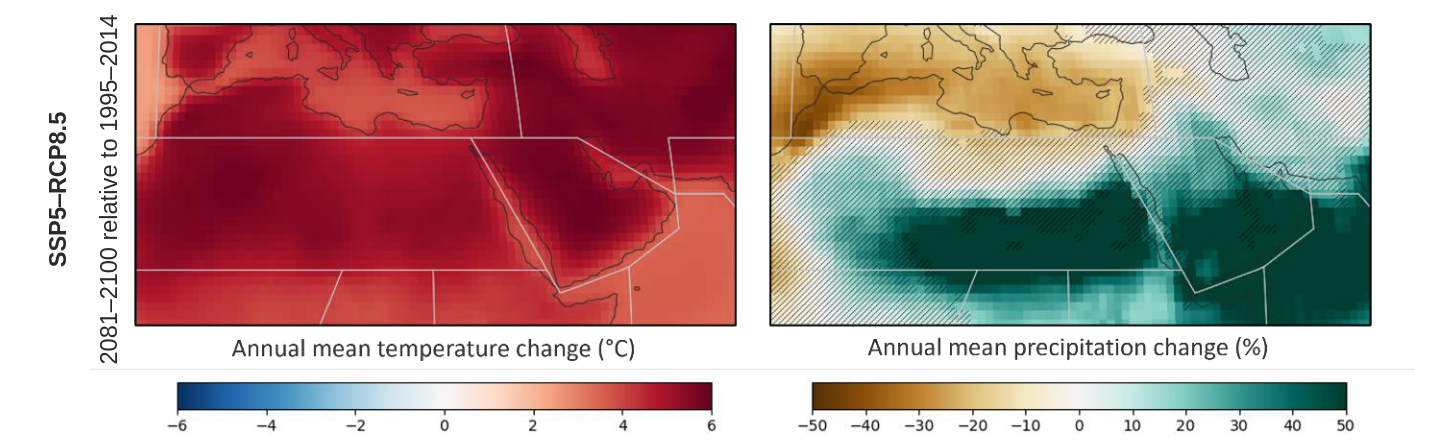
\includegraphics[scale=0.25]{actual_vs_past.png}
	\caption{Projected change in annual mean temperature (left) and annual mean precipitation
(right) between 1995–2014 and 2081–2100 under the SSP5–RCP8.5 scenario based on CMIP6
models (Gutiérrez et al., 2021). Note that precipitation change is given as a percentage: the
large increases projected over Sahara and Arabian deserts equate to only a few millimetres of
additional rainfall.}
\end{figure}



\subsubsection{Impact-Based Evaluation}
Impact-based forecasting refers to a type of weather or climate forecasting that goes beyond predicting the meteorological parameters (e.g., temperature, rainfall, wind speed) and instead focuses on predicting the potential impacts of those conditions on society, infrastructure, and ecosystems. The goal is to provide actionable insights that help communities and decision-makers prepare for and mitigate the effects of extreme weather and climate events.

\textbf{Evaluation of Seasonal Forecast Models}\\
An impact-based evaluation\footnote{\url{//www.researchgate.net/publication/385818108_Impact-Based_Skill_Evaluation_of_Seasonal_Precipitation_Forecasts}} was conducted on five seasonal forecast models to identify the most effective for precipitation forecasting. The models assessed included:
\begin{itemize}
    \item Centro Euro‐Mediterraneo sui Cambiamenti Climatici (CMCC: version 35),
    \item Deutscher Wetterdienst (DWD: version 21),
    \item Environment and Climate Change Canada (ECCC: version 3),
    \item Météo‐France (version 8),
    \item UK Met Office (UK‐Met: version 601).
\end{itemize}

The findings highlighted the \textbf{\textit{UK‐Met} }  and \textbf{\textit{Météo‐France} } models as consistently superior across all four seasons. Meanwhile, the ECCC and CMCC models exhibited strong performance on specific indices and in particular regions, ranking just below the top two models.

\textbf{ROC Scores and Regional Performance}\\
The ROC scores indicate that forecast models perform exceptionally well in tropical and subtropical regions. This result is consistent with our study and can be attributed to the general predictability of oceanic conditions and the influence of climate drivers such as the El Niño-Southern Oscillation (ENSO). The Météo‐France and UK‐Met models exhibited superior performance during the SON and MAM seasons.

However, the prevalence of grids with no discrimination ROC categories is more common in extratropical regions. This can be attributed to:
\begin{itemize}
    \item Lower predictability of extratropical variations,
    \item Model limitations in capturing interactions between tropical and extratropical regions,
    \item Challenges in representing land surface processes (De Andrade et al., 2019).
\end{itemize}
The CMCC, DWD, and ECCC models often fail to detect extreme events in many extratropical areas, underscoring the stronger performance of the UK‐Met and Météo‐France models in these scenarios.

\textbf{Percent Bias Analysis}\\
The analysis of Percent Bias across four seasons demonstrates a consistent underestimation by forecast models for most extreme wet precipitation indices. Key observations include:
\begin{itemize}
    \item Forecast models underestimate extreme wet precipitation indices while overestimating light precipitation.
    \item Models perform better in capturing the intensity and magnitude of extreme events (e.g., highest daily and multi-day rainfall) compared to the frequency of wet or dry days.
\end{itemize}

In tropical and subtropical regions, models like \textbf{\textit{UK‐Met}}  and \textbf{\textit{Météo‐France} } exhibit strong performance due to their ability to capture large-scale climate patterns. In contrast, extratropical regions show higher biases, reflecting challenges in modeling complex interactions and seasonal variations.

\textbf{Global Model Comparison}\\
The \textbf{\textit{UK‐Met}} model consistently demonstrates lower biases and stronger performance globally compared to the \textbf{\textit{Météo‐France} }  model, highlighting its effectiveness in representing climate patterns. However, all models show limitations in accurately modeling persistent extreme wet and dry periods, particularly in extratropical areas.


\subsubsection{SYSTEM 7 FRANCE}

seasonal forecasting evaluation has been the subject of numerous studies, with a focus on improving the accuracy and reliability of predictions related to precipitation and other weather parameters. One such study\footnote{https://www.mdpi.com/2674-0494/1/3/16} conducted a probabilistic evaluation of seasonal precipitation re-forecasting from May to November over a period of 23 years (1993–2015). The study utilized the Brier Score (BS) and its decomposition to assess forecast performance, with the aim of providing more reliable and actionable predictions for extreme weather events.

The evaluation was conducted on the operational seasonal forecasting system of Meteo-France, which used 25 ensemble members, perturbed model dynamics, and initial conditions. The system aimed to provide a more detailed probabilistic forecast, in addition to existing deterministic metrics, for both seasonal and intra-seasonal forecasts. The BS was estimated using tercile probabilities and a non-parametric counting estimator, with the GPCP\footnote{Global Precipitation Climatology Project (GPCP)} observation data serving as the reference.

Multiple analyses were performed to evaluate the robustness of the BS score, revealing that spatial distributions of the BS can vary significantly based on the sampling methods, reference data, and ensemble types used. The analysis showed that large errors, especially in the tropical ocean, could be reduced by using hindcast ensemble climatological samples. In particular, errors over the Nino region in the Pacific Ocean could be mitigated using these methods. This highlights the importance of employing various ensemble data sources and reference climatology to enhance the reliability of seasonal forecasts.

A notable finding was the reduction in BS when using ensemble observations, especially in the tropical ocean, suggesting that increasing ensemble size can improve forecast accuracy up to a point. However, this was not the case in all regions, as some areas, such as the tropical Indian Ocean, exhibited high BS even with different analysis methods. The study also found that intra-seasonal analyses showed similar patterns to seasonal hindcasts, but with higher BS due to reduced sample sizes, highlighting the need for higher-resolution models and improved initial conditions.

The study concluded that, despite improvements, probabilistic forecasting still faces challenges, particularly in the tropical regions, where errors fluctuate with lead time. The study emphasized the need for continued development of forecasting methods, particularly in reducing uncertainties in evaluation scores. Future evaluations should expand beyond the BS to include other metrics, such as the forecast skill score and the relative operating characteristic (ROC), to better assess forecast performance and identify system deficiencies.

This study's findings underline the importance of ensemble forecasting and the use of diverse data sources to improve the accuracy of seasonal precipitation forecasts, particularly in tropical regions where predictability remains challenging.


\subsection{Evaluation Approaches}


In the WMO\footnotemark{} \footnotetext{https://library.wmo.int/records/item/56227-guidance-on-verification-of-operational-seasonal-climate-forecasts}. Guide, several criteria are provided for evaluating a good forecast. Each criterion offers insight into specific aspects of the model but cannot, on its own, fully determine the forecast's quality. By combining all the criteria, we can comprehensively assess the performance of the model.	 
		\subsubsection{Resolution}
	Resolution measures whether the outcome differs given different forecasts, while discrimination measures whether the forecasts differ given different outcomes.

Discrimination looks at how well your forecast separates cases when the event (outcome) happens (pass) from when it doesn’t happen (fail). It’s about telling apart the events.
Resolution looks at how well your forecast adapts to different situations, giving distinct probabilities for different cases. It’s about adjusting to the situation.

Resolution measures how well a forecast distinguishes between different outcomes. A forecast has high resolution if the predicted probabilities vary significantly depending on the actual outcome. In other words, resolution tells us whether the forecast changes (e.g., gives different probabilities) when the actual outcome changes.
High resolution: The forecast gives distinct and varying probabilities when different events (outcomes) occur. For example, if in one case the forecast predicts a high probability of rain and it rains, and in another case predicts a low probability and it doesn’t rain, the forecast shows good resolution.
Low resolution: If the forecast probabilities don’t change much regardless of whether it rains or not (e.g., always predicting a 50\% chance of rain), the forecast has poor resolution because it fails to capture the differences in actual outcomes.
Resolution can be determined by measuring how strongly the outcome is conditioned upon the forecast.
If the outcome is independent of the forecast, the forecast has no resolution and is useless
Forecasts with no resolution are neither “good” nor “bad”, but are useless. 
Metrics of resolution distinguish between potentially useful and useless forecasts, but not all these metrics distinguish between “good” and “bad” forecasts.

The following equation represents the "resolution" component of the Brier Score (BS) decomposition, which quantifies how well a set of probability forecasts differentiates between events and non-events:

\begin{equation}
\textbf {Resolution} = \frac{1}{n} \sum_{k=1}^{d} n_k \left( \bar{y}_k - \bar{y} \right)^2
\end{equation}

where:

\begin{equation}
\bar{y}_k = \frac{1}{n_k} \sum_{i=1}^{n_k} y_{k,i}
\end{equation}

\begin{itemize}
    \item $n$ is the total number of forecasts,
    \item $d$ is the number of discrete probability bins,
    \item $n_k$ is the number of forecasts in the $k$-th bin,
    \item $\bar{y}_k$ is the observed relative frequency for the $k$-th probability bin,
    \item $\bar{y}$ is the overall observed relative frequency.
\end{itemize}

The term $\left( \bar{y}_k - \bar{y} \right)^2$ captures the variance between individual forecast categories and the overall event frequency. Higher resolution indicates that forecasts better differentiate between events and non-events.\\
so the resolution tells us how the model change with different situations.\\
the scores used to evaluate resolution are Brier Score and Reliability.



		\subsubsection{Discrimination}

Discrimination measures how well the forecast separates cases where the event occurs from cases where it does not. In other words, it examines whether the forecast probabilities differ for events that happen versus those that don't.
High discrimination: A forecast has high discrimination if, for example, when rain occurs, the forecast consistently predicts a high probability of rain, and when rain doesn’t occur, it predicts a low probability. It means the forecast is good at distinguishing between rain and no-rain days.
Low discrimination: If the forecast provides similar probabilities regardless of whether it rains or not (e.g., predicting a 60\% chance of rain every day), it has poor discrimination because it doesn’t effectively differentiate between days with and without rain. The score used to evaluate descrimination is ROC\footnote{Relative operating characteristics}.
		\subsubsection{Reliability}

A forecast is reliable if the predicted probabilities match the actual frequencies. For instance:
If you forecast a 40\% probability for below-normal rainfall, below-normal rainfall should occur in 40\% of the cases where you make that prediction.
Similarly, if you forecast a 25\% chance of above-normal rainfall, above-normal rainfall should happen 25\% of the time when you give that probability.
If this relationship holds consistently over many forecasts, the forecasts are well-calibrated (or reliable).
A Reliable but Uninformative Forecast
A forecast that always gives the climatological probability (e.g., always predicting a 33\% chance for each category: below, normal, above normal) would be reliable because the climatological average matches the observed frequencies. However, this forecast wouldn’t provide any information about changing conditions from case to case—it doesn’t adapt to the current situation, making it uninformative.

\begin{equation}
\textbf{Reliability} = \frac{1}{n} \sum_{k=1}^{d} n_k \left( \bar{p}_k - \bar{y}_k \right)^2
\end{equation}


\begin{itemize}
    \item $n$ is the total number of forecasts,
    \item $d$ is the number of discrete probability bins,
    \item $n_k$ is the number of forecasts in the $k$-th bin,
    \item $\bar{y}_k$ is the observed relative frequency for the $k$-th probability bin,
    \item $\bar{p}_k$ is relative frequency for the $k$-th probability.
\end{itemize}


		\subsubsection{Sharpness}
Sharp forecasts provide a strong signal about the expected outcome. For example, a sharp forecast might assign a 70\% chance to a certain outcome, like above-normal rainfall. This high probability communicates more confidence in that specific outcome.
On the other hand, when the forecast probabilities are close to the climatological values (like assigning a 40\% chance to above-normal, 35\% to normal, and 25\% to below-normal), the forecast is not very sharp, meaning the forecaster isn't very confident in predicting any one outcome.
The climatological probabilities are reliable, but aren’t sharp.
